\documentclass[11pt]{article}

% ——— Standard Packages ———
\usepackage{amsmath,amssymb}
\usepackage{graphicx}
\usepackage[margin=1in]{geometry}
\usepackage{setspace}
\usepackage{cite}
\usepackage[colorlinks=true,linkcolor=blue,citecolor=blue,urlcolor=blue]{hyperref}
\usepackage{appendix}
\usepackage[hang,flushmargin]{footmisc}
\usepackage{caption}
\usepackage{float}
\usepackage{minipage-marginpar}
\usepackage{bm} % for bold math symbols



\newcommand{\sgn}{\mathrm{sign}}

% ——— Caption Setup ———
\captionsetup{font=footnotesize,labelfont=bf}

%
\begin{document}

% ——— All‐in‐One Centered Header ———
\begin{center}
  \huge\bfseries
  Emergent Relativistic Phenomena in Condensed Matter
\end{center}
\begin{center}
  \normalsize
  Harry Luo\\[0.1ex]
  Physics 531 Honors Project, May 2025
\end{center}


\begin{abstract}
  This paper explores emergent relativistic phenomena in condensed matter systems modeled by Dirac Hamiltonians. We investigate the spectral properties of 1D, 2D, and 3D bulk Dirac equations, deriving their energy eigenvalues and eigenstates. For the 2D massive Dirac Hamiltonian, we calculate the Berry connection and Berry curvature, leading to the determination of the Chern number $C = \frac{1}{2}\sgn(m)$. Subsequently, we analyze the formation of Landau levels for this 2D system in a perpendicular magnetic field. The characteristic $\sqrt{nB}$ energy scaling for $n \ge 1$ levels and the unique $n=0$ level at $E_0 = m \sgn(qB)$ are derived. The orbital degeneracy of these levels is determined, and the spectrum's dependence on the mass gap is discussed. Finally, the electron density at half-filling ($\mu=0$) is calculated, $\bar{n}_0 = -\sgn(qBm) |qB|/(4\pi)$, along with its derivative with respect to the magnetic field, $d\bar{n}_0/dB = -q \sgn(m)/(4\pi)$, highlighting key features relevant to transport phenomena in Dirac materials.
  \end{abstract}
  
  \vspace{0.5cm} % Optional: adds a little space before the first section
  


\section{Bulk Dirac Equation}\subsection{1D Dirac Hamiltonian}

The Hamiltonian is given by:
\begin{equation}
H_{0} = v \hat{p}_x \sigma_x + m \sigma_z,
\end{equation}
where $\hat{p}_x = -i \frac{\partial}{\partial x}$, $v$ is a velocity parameter, $m$ is the mass, and $\sigma_x, \sigma_z$ are Pauli matrices. We work in units where $\hbar=1$.

\textbf{Fourier Transformation:}
We transform to momentum space by considering plane wave solutions $\psi(x) = e^{ipx} \psi(p)$. The momentum operator $\hat{p}_x$ becomes multiplication by $p$. The Hamiltonian in momentum space is:
\begin{equation}
H_0(p) = v p \sigma_x + m \sigma_z = \begin{pmatrix} m & v p \\ v p & -m \end{pmatrix}.
\end{equation}

\textbf{Eigenvalues:}
The energy eigenvalues $E(p)$ are found by solving $\det(H_0(p) - E I) = 0$:
\[ \det \begin{pmatrix} m - E & v p \\ v p & -m - E \end{pmatrix} = -(m^2 - E^2) - (v p)^2 = 0 \]
\[ E^2 = m^2 + (v p)^2 \]
The eigenvalues form two energy bands:
\begin{equation}
E_{\pm}(p) = \pm \sqrt{m^2 + (v p)^2}.
\label{eq:1D_eigenvalues}
\end{equation}
Let $E_+(p) = \sqrt{m^2 + (v p)^2}$ be the magnitude.


\textbf{Eigenstates:}
We solve $(H_0(p) - E_{\pm} I) \psi_{\pm}(p) = 0$ for the eigenstates $\psi_{\pm}(p)$.
For the positive energy $E = E_+(p)$, the normalized eigenstate is:
\begin{equation}
\psi_+(p) = \frac{1}{\sqrt{2 E_+(p) (E_+(p) + m)}} \begin{pmatrix} E_+(p) + m \\ v p \end{pmatrix}.
\label{eq:1D_eigenstate_plus}
\end{equation}
For the negative energy $E = E_-(p) = -E_+(p)$, the normalized eigenstate is:
\begin{equation}
\psi_-(p) = \frac{1}{\sqrt{2 E_+(p) (E_+(p) + m)}} \begin{pmatrix} -v p \\ E_+(p) + m \end{pmatrix}.
\label{eq:1D_eigenstate_minus}
\end{equation}
These states are orthogonal and normalized, $\psi_{\lambda}^\dagger(p) \psi_{\lambda'}(p) = \delta_{\lambda \lambda'}$.

\textbf{Dispersion Relation:}
The energy eigenvalues $E_{\pm}(p)$ given by \eqref{eq:1D_eigenvalues} are plotted versus momentum $p$ in Figure \ref{fig:1D_dispersion}. The plot shows the characteristic hyperbolic bands for a massive particle (solid lines, $m=1$) with an energy gap $2m$ at $p=0$, and the linear bands touching at a \textbf{Dirac point} for a massless particle (dashed lines, $m=0$).

\begin{figure}[htbp] % h=here, t=top, b=bottom, p=page of floats
    \centering
    % Make sure graphicx package is loaded: \usepackage{graphicx}
    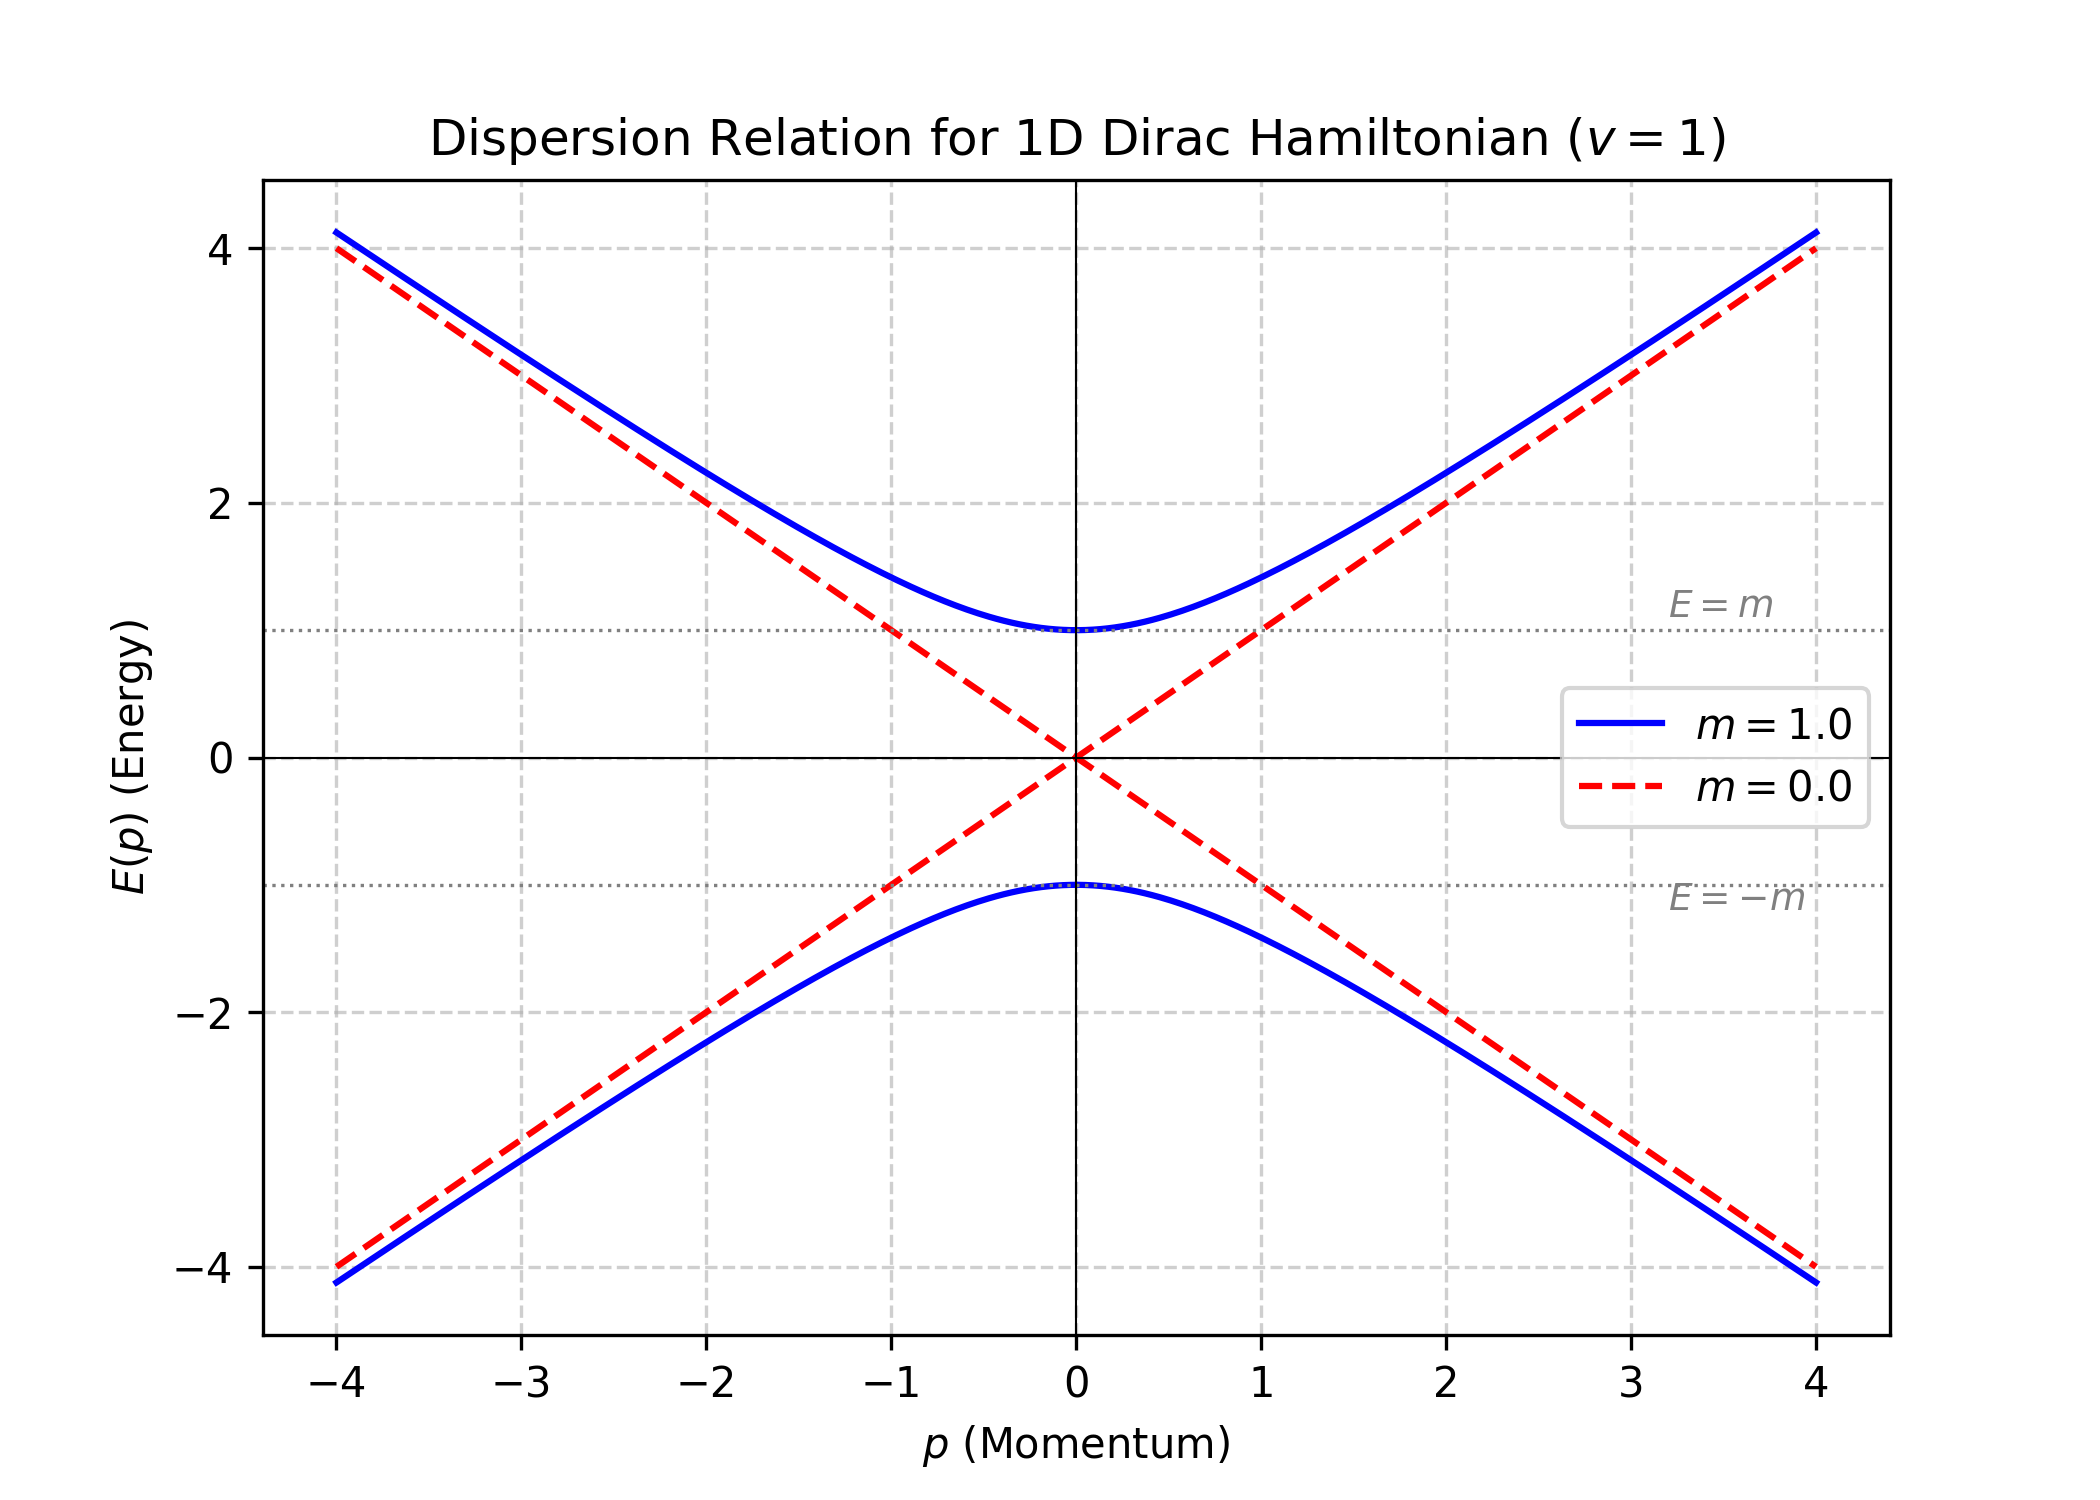
\includegraphics[width=0.7\textwidth]{1d_dirac_dispersion.png} % Ensure this matches the filename
    \caption{Dispersion relation $E_{\pm}(p) = \pm \sqrt{m^2 + (v p)^2}$ for the 1D Dirac Hamiltonian \eqref{eq:1D_eigenvalues}, with $v=1$. The solid lines show the gapped case ($m=1$), illustrating the energy gap of $2m$ at $p=0$. The dashed lines show the gapless case ($m=0$), where the bands touch at a Dirac point at $(p,E)=(0,0)$ and the dispersion is linear $E=\pm v|p|$.}
    \label{fig:1D_dispersion}
\end{figure}


\subsection{2D Dirac Hamiltonian}

We then consider the standard 2D massive Dirac Hamiltonian:
\begin{equation}
H_{0} = v (\hat{p}_x \sigma_x + \hat{p}_y \sigma_y) + m \sigma_z,
\end{equation}
where $\hat{\mathbf{p}} = (\hat{p}_x, \hat{p}_y) = (-i \partial_x, -i \partial_y)$, $v$ is the velocity parameter, $m$ is the mass, and $\sigma_{x,y,z}$ are the Pauli matrices. We set $\hbar=1$.

\textbf{Fourier Transformation:}
Transforming to momentum space $\mathbf{p} = (p_x, p_y)$, the Hamiltonian becomes a $2 \times 2$ matrix:
\begin{align} H_0(\mathbf{p}) &= v (p_x \sigma_x + p_y \sigma_y) + m \sigma_z \\ &= v p_x \begin{pmatrix} 0 & 1 \\ 1 & 0 \end{pmatrix} + v p_y \begin{pmatrix} 0 & -i \\ i & 0 \end{pmatrix} + m \begin{pmatrix} 1 & 0 \\ 0 & -1 \end{pmatrix} \\ &= \begin{pmatrix} m & v p_x - i v p_y \\ v p_x + i v p_y & -m \end{pmatrix} \\ &= \begin{pmatrix} m & v(p_x - i p_y) \\ v(p_x + i p_y) & -m \end{pmatrix}. \label{eq:2D_H_matrix}\end{align}

\textbf{Eigenvalues:}
We find the eigenvalues $E(\mathbf{p})$ by solving $\det(H_0(\mathbf{p}) - E I) = 0$:
\[ \det \begin{pmatrix} m - E & v(p_x - i p_y) \\ v(p_x + i p_y) & -m - E \end{pmatrix} = 0 \]
\[ (m - E)(-m - E) - v^2 (p_x + i p_y)(p_x - i p_y) = 0 \]
\[ -(m^2 - E^2) - v^2 (p_x^2 + p_y^2) = 0 \]
Let $p = |\mathbf{p}| = \sqrt{p_x^2 + p_y^2}$ be the magnitude of the momentum.
\[ E^2 = m^2 + v^2 p^2 \]
The energy eigenvalues are:
\begin{equation}
E_{\pm}(p) = \pm \sqrt{m^2 + v^2 p^2}.
\label{eq:2D_eigenvalues}
\end{equation}
Let $E_+(p) = \sqrt{m^2 + v^2 p^2}$ be the positive energy magnitude.

\textbf{Eigenstates:}
We solve $(H_0(\mathbf{p}) - E_{\pm} I) \psi_{\pm}(\mathbf{p}) = 0$ for the normalized eigenstates $\psi_{\pm}(\mathbf{p})$.
For the positive energy $E = E_+(p)$:
\begin{equation}
\psi_+(\mathbf{p}) = \frac{1}{\sqrt{2 E_+(p) (E_+(p) + m)}} \begin{pmatrix} m + E_+(p) \\ v(p_x + i p_y) \end{pmatrix}.
\label{eq:2D_eigenstate_plus}
\end{equation}
For the negative energy $E = E_-(p) = -E_+(p)$:
\begin{equation}
\psi_-(\mathbf{p}) = \frac{1}{\sqrt{2 E_+(p) (E_+(p) + m)}} \begin{pmatrix} v(p_x - i p_y) \\ -(m + E_+(p)) \end{pmatrix}.
\label{eq:2D_eigenstate_minus}
\end{equation}
These states are orthogonal and normalized. In polar coordinates $(p, \phi)$, where $p_x = p \cos \phi$ and $p_y = p \sin \phi$, we have $p_x \pm i p_y = p e^{\pm i \phi}$. The eigenstates depend on both the magnitude $p$ and the angle $\phi$ of the momentum vector:
\begin{equation}
\psi_+(p, \phi) = \frac{1}{\sqrt{2 E_+(p) (E_+(p) + m)}} \begin{pmatrix} m + E_+(p) \\ v p e^{i\phi} \end{pmatrix},
\end{equation}
\begin{equation}
\psi_-(p, \phi) = \frac{1}{\sqrt{2 E_+(p) (E_+(p) + m)}} \begin{pmatrix} v p e^{-i\phi} \\ -(m + E_+(p)) \end{pmatrix}.
\end{equation}

\textbf{Dispersion Relation:}
The energy eigenvalues $E_{\pm}(\mathbf{p})$ depend only on the magnitude $p=|\mathbf{p}|$ as given in \eqref{eq:2D_eigenvalues}. Since the momentum space is two-dimensional $(p_x, p_y)$, the dispersion is visualized as surfaces in 3D, shown in Figures \ref{fig:2D_dispersion_gapped} and \ref{fig:2D_dispersion_gapless}.

For a non-zero mass ($m \neq 0$), the energy bands form two hyperboloid sheets symmetric around the energy axis and separated by a gap of $2|m|$ at $\mathbf{p}=0$ (Figure \ref{fig:2D_dispersion_gapped}).

In the massless case ($m=0$), the gap closes, and the dispersion $E_{\pm}(\mathbf{p}) = \pm v |\mathbf{p}|$ forms the distinctive \textbf{Dirac cone} structure, where the upper and lower bands meet at a single point (the Dirac point) at the origin (Figure \ref{fig:2D_dispersion_gapless}).
\begin{figure}[htbp]
  \centering
  \begin{minipage}[t]{0.48\textwidth}
    \centering
    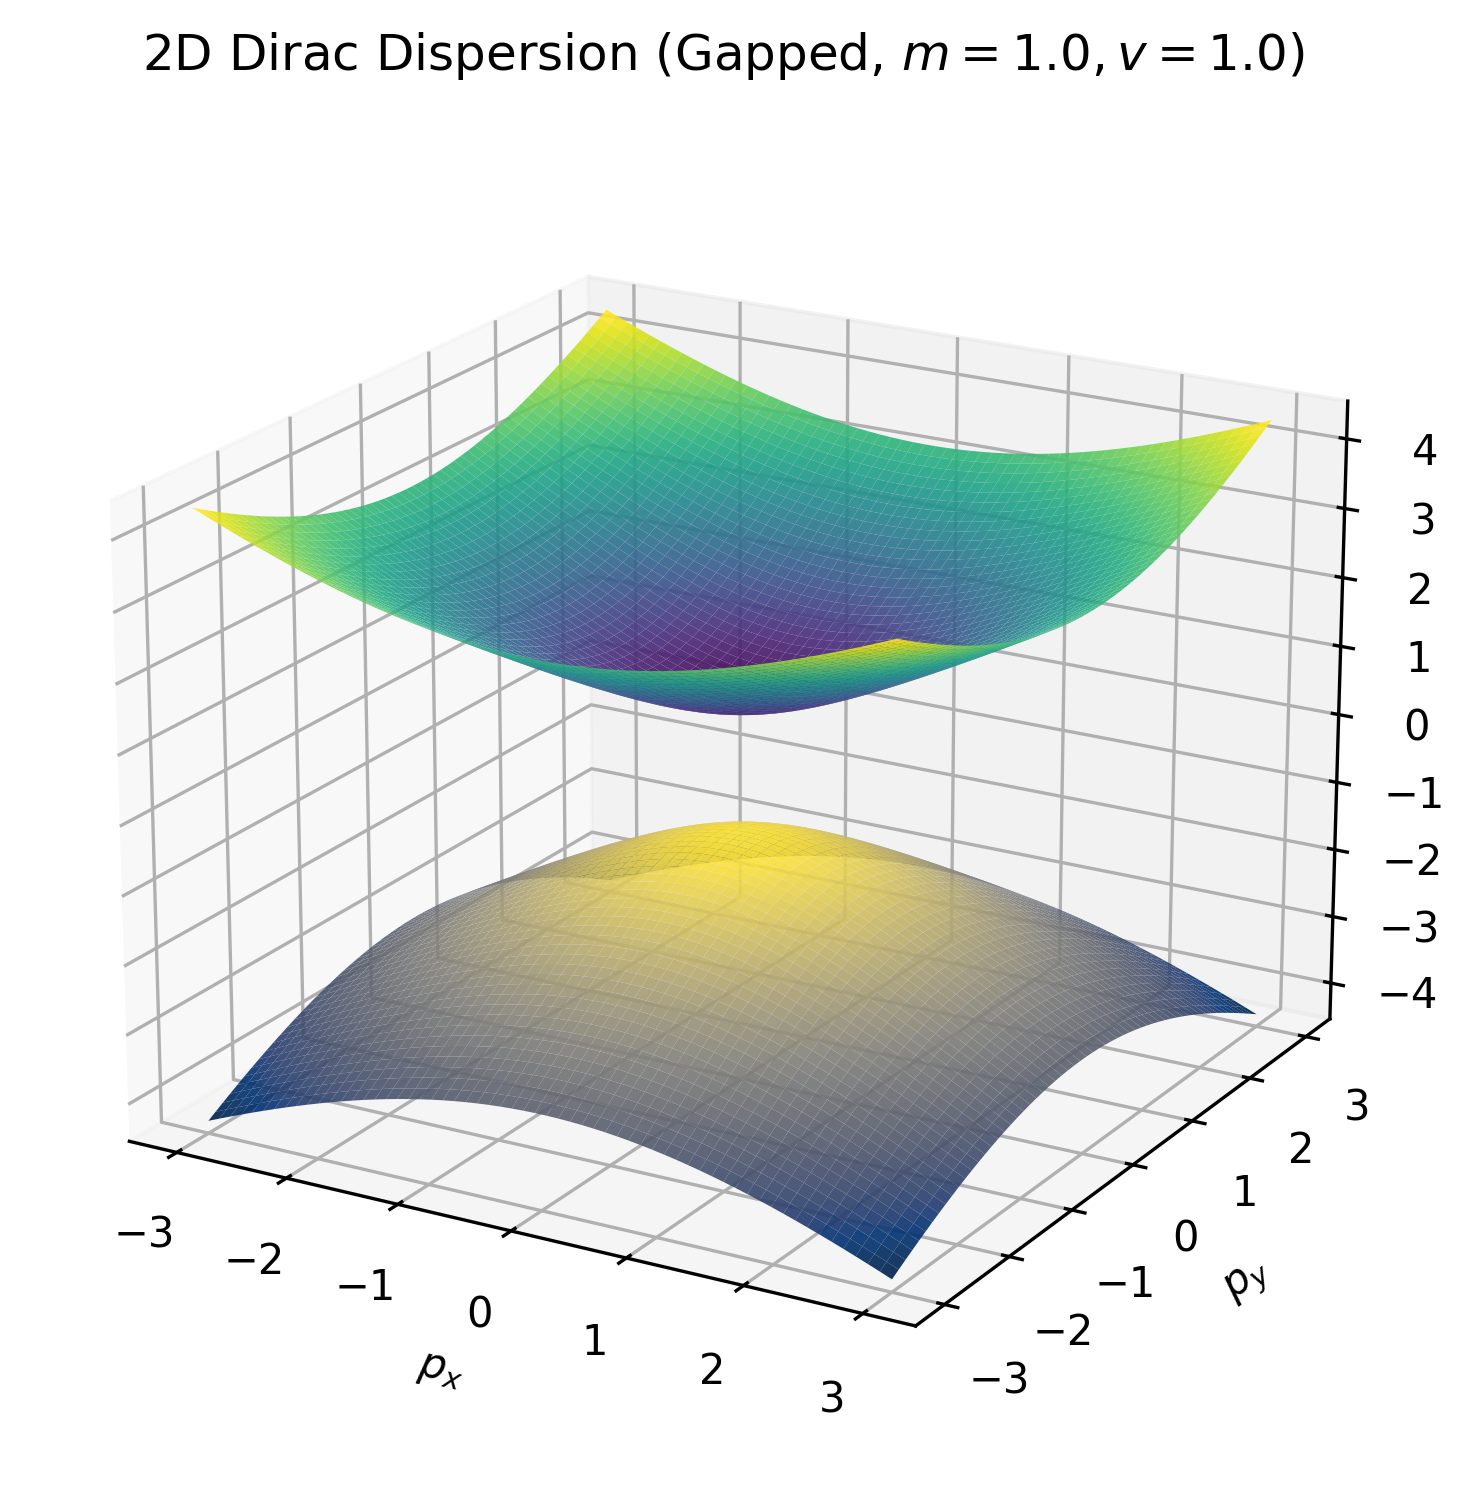
\includegraphics[width=\textwidth]{2d_dirac_dispersion_gapped.png}
    \caption{3D plot of the dispersion relation $E_{\pm}(\mathbf{p}) = \pm \sqrt{m^2 + v^2(p_x^2+p_y^2)}$ for the 2D massive Dirac Hamiltonian \eqref{eq:2D_eigenvalues} ($m=1, v=1$). The plot shows two hyperboloid sheets separated by a gap $2m$ at $\mathbf{p}=0$.}
    \label{fig:2D_dispersion_gapped}
  \end{minipage}
  \hfill
  \begin{minipage}[t]{0.48\textwidth}
    \centering
    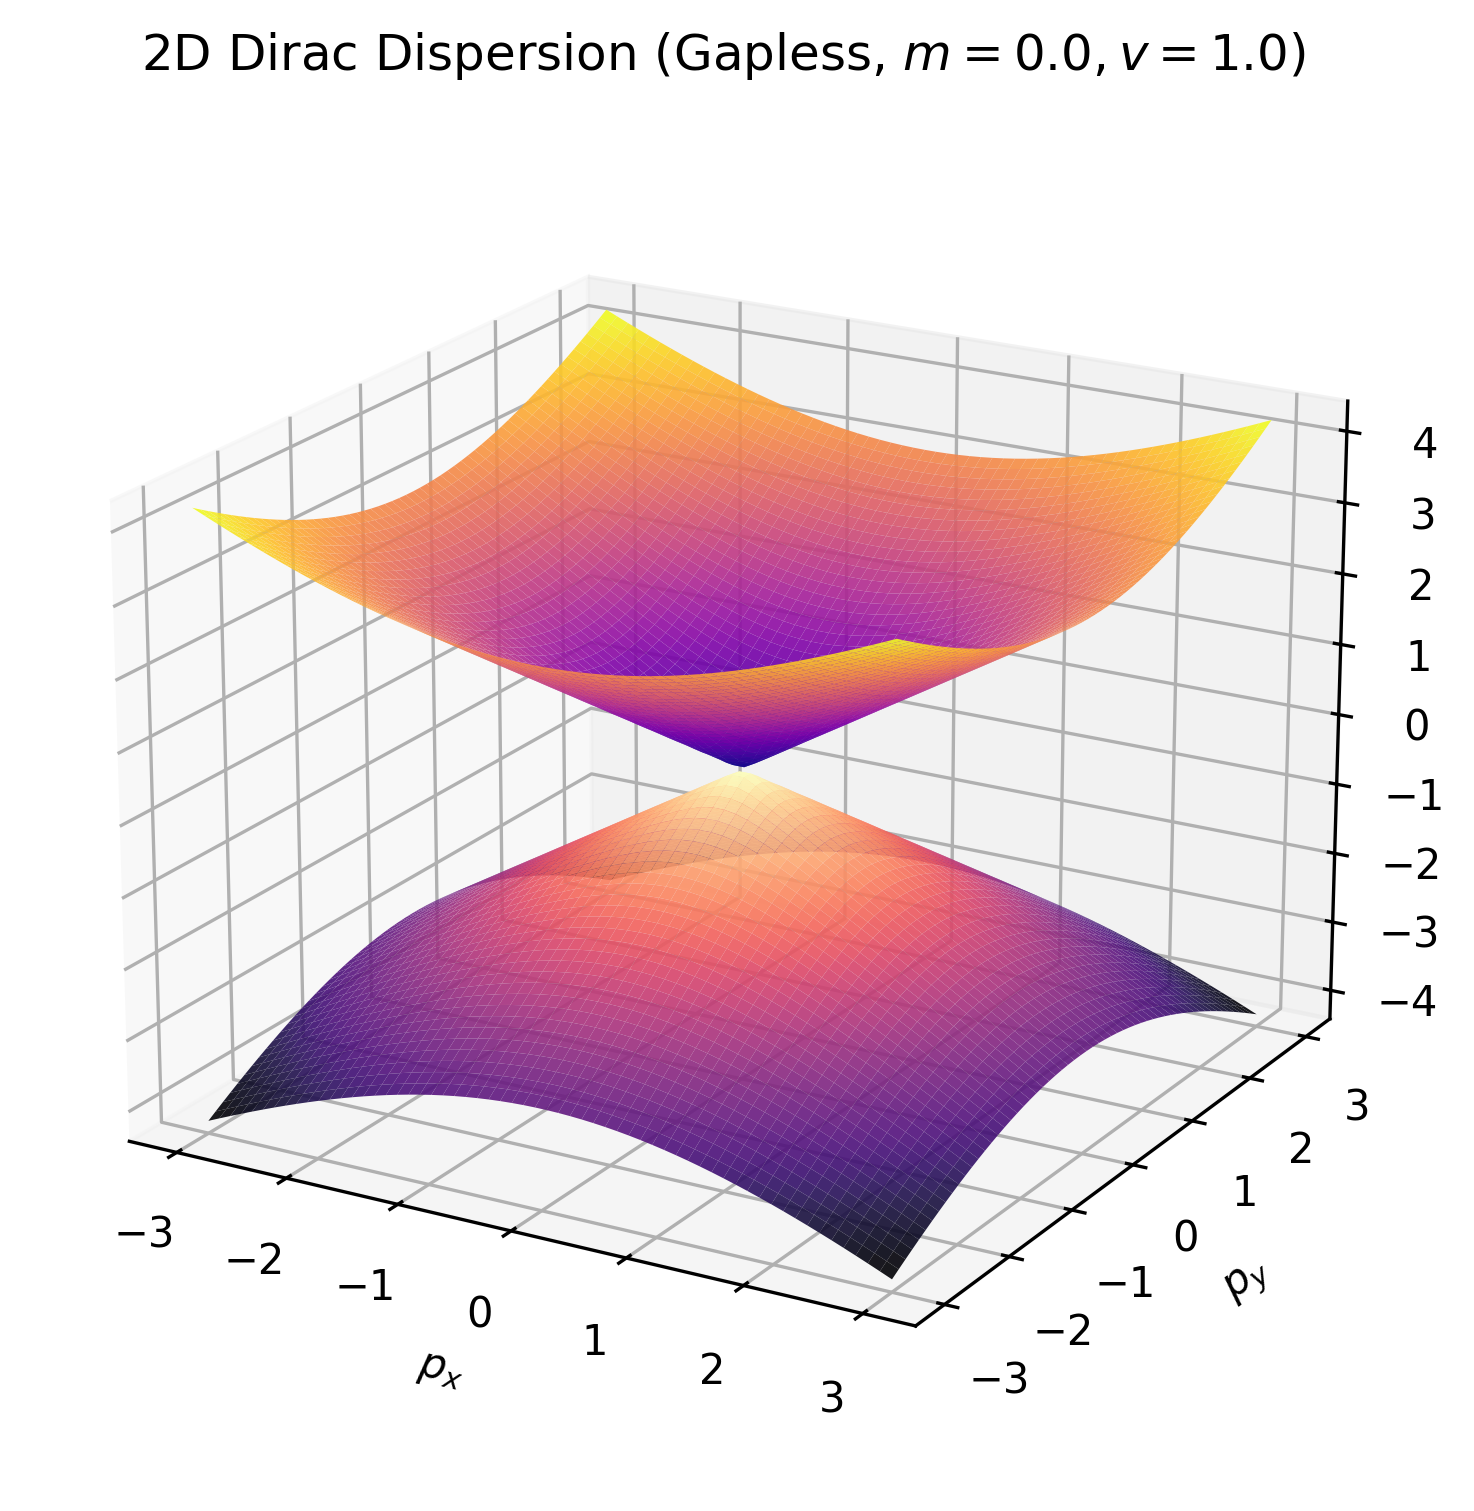
\includegraphics[width=\textwidth]{2d_dirac_dispersion_gapless.png}
    \caption{3D plot of the dispersion relation $E_{\pm}(\mathbf{p}) = \pm v |\mathbf{p}|$ for the 2D massless Dirac Hamiltonian \eqref{eq:2D_eigenvalues} ($m=0, v=1$). The plot shows the characteristic \textbf{Dirac cone} structure, with the bands meeting at the Dirac point $(E=0, \mathbf{p}=0)$.}
    \label{fig:2D_dispersion_gapless}
  \end{minipage}
\end{figure}



\subsection{3D Dirac Hamiltonian}

The Hamiltonian is given in the form:
\begin{equation}
H_0 = v(\hat{p}_x \beta_x + \hat{p}_y \beta_y + \hat{p}_z \beta_z) + m \alpha = v (\hat{\mathbf{p}} \cdot \bm{\beta}) + m \alpha,
\end{equation}
where $\hat{\mathbf{p}} = (\hat{p}_x, \hat{p}_y, \hat{p}_z)$ is the momentum operator, $v$ is the velocity parameter, $m$ is the mass, and $\beta_x, \beta_y, \beta_z, \alpha$ are mutually anti-commuting matrices satisfying $\beta_i^2 = \alpha^2 = I$. These are typically $4 \times 4$ Dirac matrices. We set $\hbar=1$.

\textbf{Fourier Transformation:}
In momentum space $\mathbf{p} = (p_x, p_y, p_z)$, the Hamiltonian is:
\begin{equation}
H_0(\mathbf{p}) = v (\mathbf{p} \cdot \bm{\beta}) + m \alpha.
\label{eq:3D_H_project}
\end{equation}

\textbf{Eigenvalues:}
We can find the eigenvalues by squaring the Hamiltonian. Using the Clifford algebra properties $\{\beta_i, \beta_j\} = 2 \delta_{ij} I$ and $\{\beta_i, \alpha\} = 0$:
\begin{align} H_0(\mathbf{p})^2 &= (v (\mathbf{p} \cdot \bm{\beta}) + m \alpha)^2 \\ &= v^2 (\mathbf{p} \cdot \bm{\beta})^2 + m^2 \alpha^2 + vm ((\mathbf{p} \cdot \bm{\beta})\alpha + \alpha(\mathbf{p} \cdot \bm{\beta})) \\ &= v^2 \sum_{i,j} p_i p_j \beta_i \beta_j + m^2 I + vm \sum_i p_i \{\beta_i, \alpha\} \\ &= v^2 \sum_i p_i^2 \beta_i^2 + v^2 \sum_{i<j} p_i p_j \{\beta_i, \beta_j\} + m^2 I + 0 \\ &= v^2 |\mathbf{p}|^2 I + 0 + m^2 I \\ &= (v^2 |\mathbf{p}|^2 + m^2) I. \end{align}
Since $H_0^2 \psi = E^2 \psi$, the eigenvalues $E(\mathbf{p})$ must satisfy $E^2 = v^2 |\mathbf{p}|^2 + m^2$. Letting $p = |\mathbf{p}|$:
\begin{equation}
E_{\pm}(p) = \pm \sqrt{m^2 + v^2 p^2}.
\label{eq:3D_eigenvalues}
\end{equation}
Each eigenvalue is degenerate. For $4 \times 4$ matrices, we expect two positive energy states and two negative energy states for each $\mathbf{p} \neq 0$. Let $E_+(p) = \sqrt{m^2 + v^2 p^2}$.

\textbf{Eigenstates:}
To find the eigenstates, we choose a specific representation for the matrices.We can adapt the standard Dirac-Pauli representation by mapping the matrices according to their roles in Eq. \eqref{eq:3D_H_project}:
\[ \alpha = \begin{pmatrix} I_2 & 0 \\ 0 & -I_2 \end{pmatrix}, \quad \beta_i = \begin{pmatrix} 0 & \sigma_i \\ \sigma_i & 0 \end{pmatrix}, \]
where $I_2$ is the $2 \times 2$ identity matrix and $\sigma_i$ are the Pauli matrices. Let the 4-component spinor be $\psi = \begin{pmatrix} \phi \\ \chi \end{pmatrix}$, where $\phi, \chi$ are 2-component spinors. The eigenvalue equation $H_0(\mathbf{p}) \psi = E \psi$ becomes:
\[ \begin{pmatrix} m I_2 & v (\mathbf{p} \cdot \bm{\sigma}) \\ v (\mathbf{p} \cdot \bm{\sigma}) & -m I_2 \end{pmatrix} \begin{pmatrix} \phi \\ \chi \end{pmatrix} = E \begin{pmatrix} \phi \\ \chi \end{pmatrix}. \]
This yields the coupled equations:
\begin{align} m \phi + v (\mathbf{p} \cdot \bm{\sigma}) \chi &= E \phi \label{eq:3D_coupled1} \\ v (\mathbf{p} \cdot \bm{\sigma}) \phi - m \chi &= E \chi \label{eq:3D_coupled2} \end{align}
From \eqref{eq:3D_coupled2}, $\chi = \frac{v (\mathbf{p} \cdot \bm{\sigma})}{E + m} \phi$. Substituting into \eqref{eq:3D_coupled1} recovers the eigenvalue condition $E^2 = m^2 + v^2 p^2$, using $(\mathbf{p} \cdot \bm{\sigma})^2 = |\mathbf{p}|^2 I_2$.

Let $\phi_s(\hat{\mathbf{p}})$ be the normalized 2-component eigenstate of the helicity operator $\hat{\mathbf{p}} \cdot \bm{\sigma}$ with eigenvalue $s = \pm 1$. (Note $\hat{\mathbf{p}} = \mathbf{p}/p$). Then $(\mathbf{p} \cdot \bm{\sigma}) \phi_s = p s \phi_s$.
The normalized 4-component eigenstates are constructed as follows:
For positive energy $E = E_+(p)$:
\begin{equation}
\psi_{+, s}(\mathbf{p}) = \sqrt{\frac{E_+ + m}{2 E_+}} \begin{pmatrix} \phi_s(\hat{\mathbf{p}}) \\ \frac{v p s}{E_+ + m} \phi_s(\hat{\mathbf{p}}) \end{pmatrix}, \quad s = \pm 1.
\label{eq:3D_eigenstate_plus}
\end{equation}
For negative energy $E = E_-(p) = -E_+(p)$:
\begin{equation}
\psi_{-, s}(\mathbf{p}) = \sqrt{\frac{E_+ + m}{2 E_+}} \begin{pmatrix} \frac{-v p s}{E_+ + m} \phi_s(\hat{\mathbf{p}}) \\ \phi_s(\hat{\mathbf{p}}) \end{pmatrix}, \quad s = \pm 1.
\label{eq:3D_eigenstate_minus}
\end{equation}
There are two degenerate states for each energy $E_{\pm}$ corresponding to the two helicity states $s = \pm 1$.

\textbf{Dispersion Relation:}
The energy eigenvalues $E_{\pm}(p)$ depend only on the magnitude of the 3D momentum vector $p=|\mathbf{p}|$, as given in \eqref{eq:3D_eigenvalues}. The functional form $E_{\pm}(p) = \pm \sqrt{m^2 + v^2 p^2}$ is then identical to that of the 1D case when plotted against the momentum magnitude $p$. This relationship is illustrated with updated descriptive texts in Figure \ref{fig:3D_dispersion}.

Crucially, for the 3D Hamiltonian, each energy level $E_{\pm}(p)$ (for $p \neq 0$) is doubly degenerate, corresponding to the two possible helicity states $s=\pm 1$. For $m \neq 0$ (solid lines), the plot shows the gapped spectrum with two degenerate bands separated by $2|m|$ at $p=0$. For $m=0$ (dashed lines), the gap closes at the origin, forming a 3D Dirac point where the linear dispersion bands $E_{\pm}(p) = \pm v p$ meet.

\begin{figure}[htbp]
    \centering
    % Reusing the 1D plot figure, as E vs |p| is the same shape.
    % Make sure graphicx package is loaded: \usepackage{graphicx}
    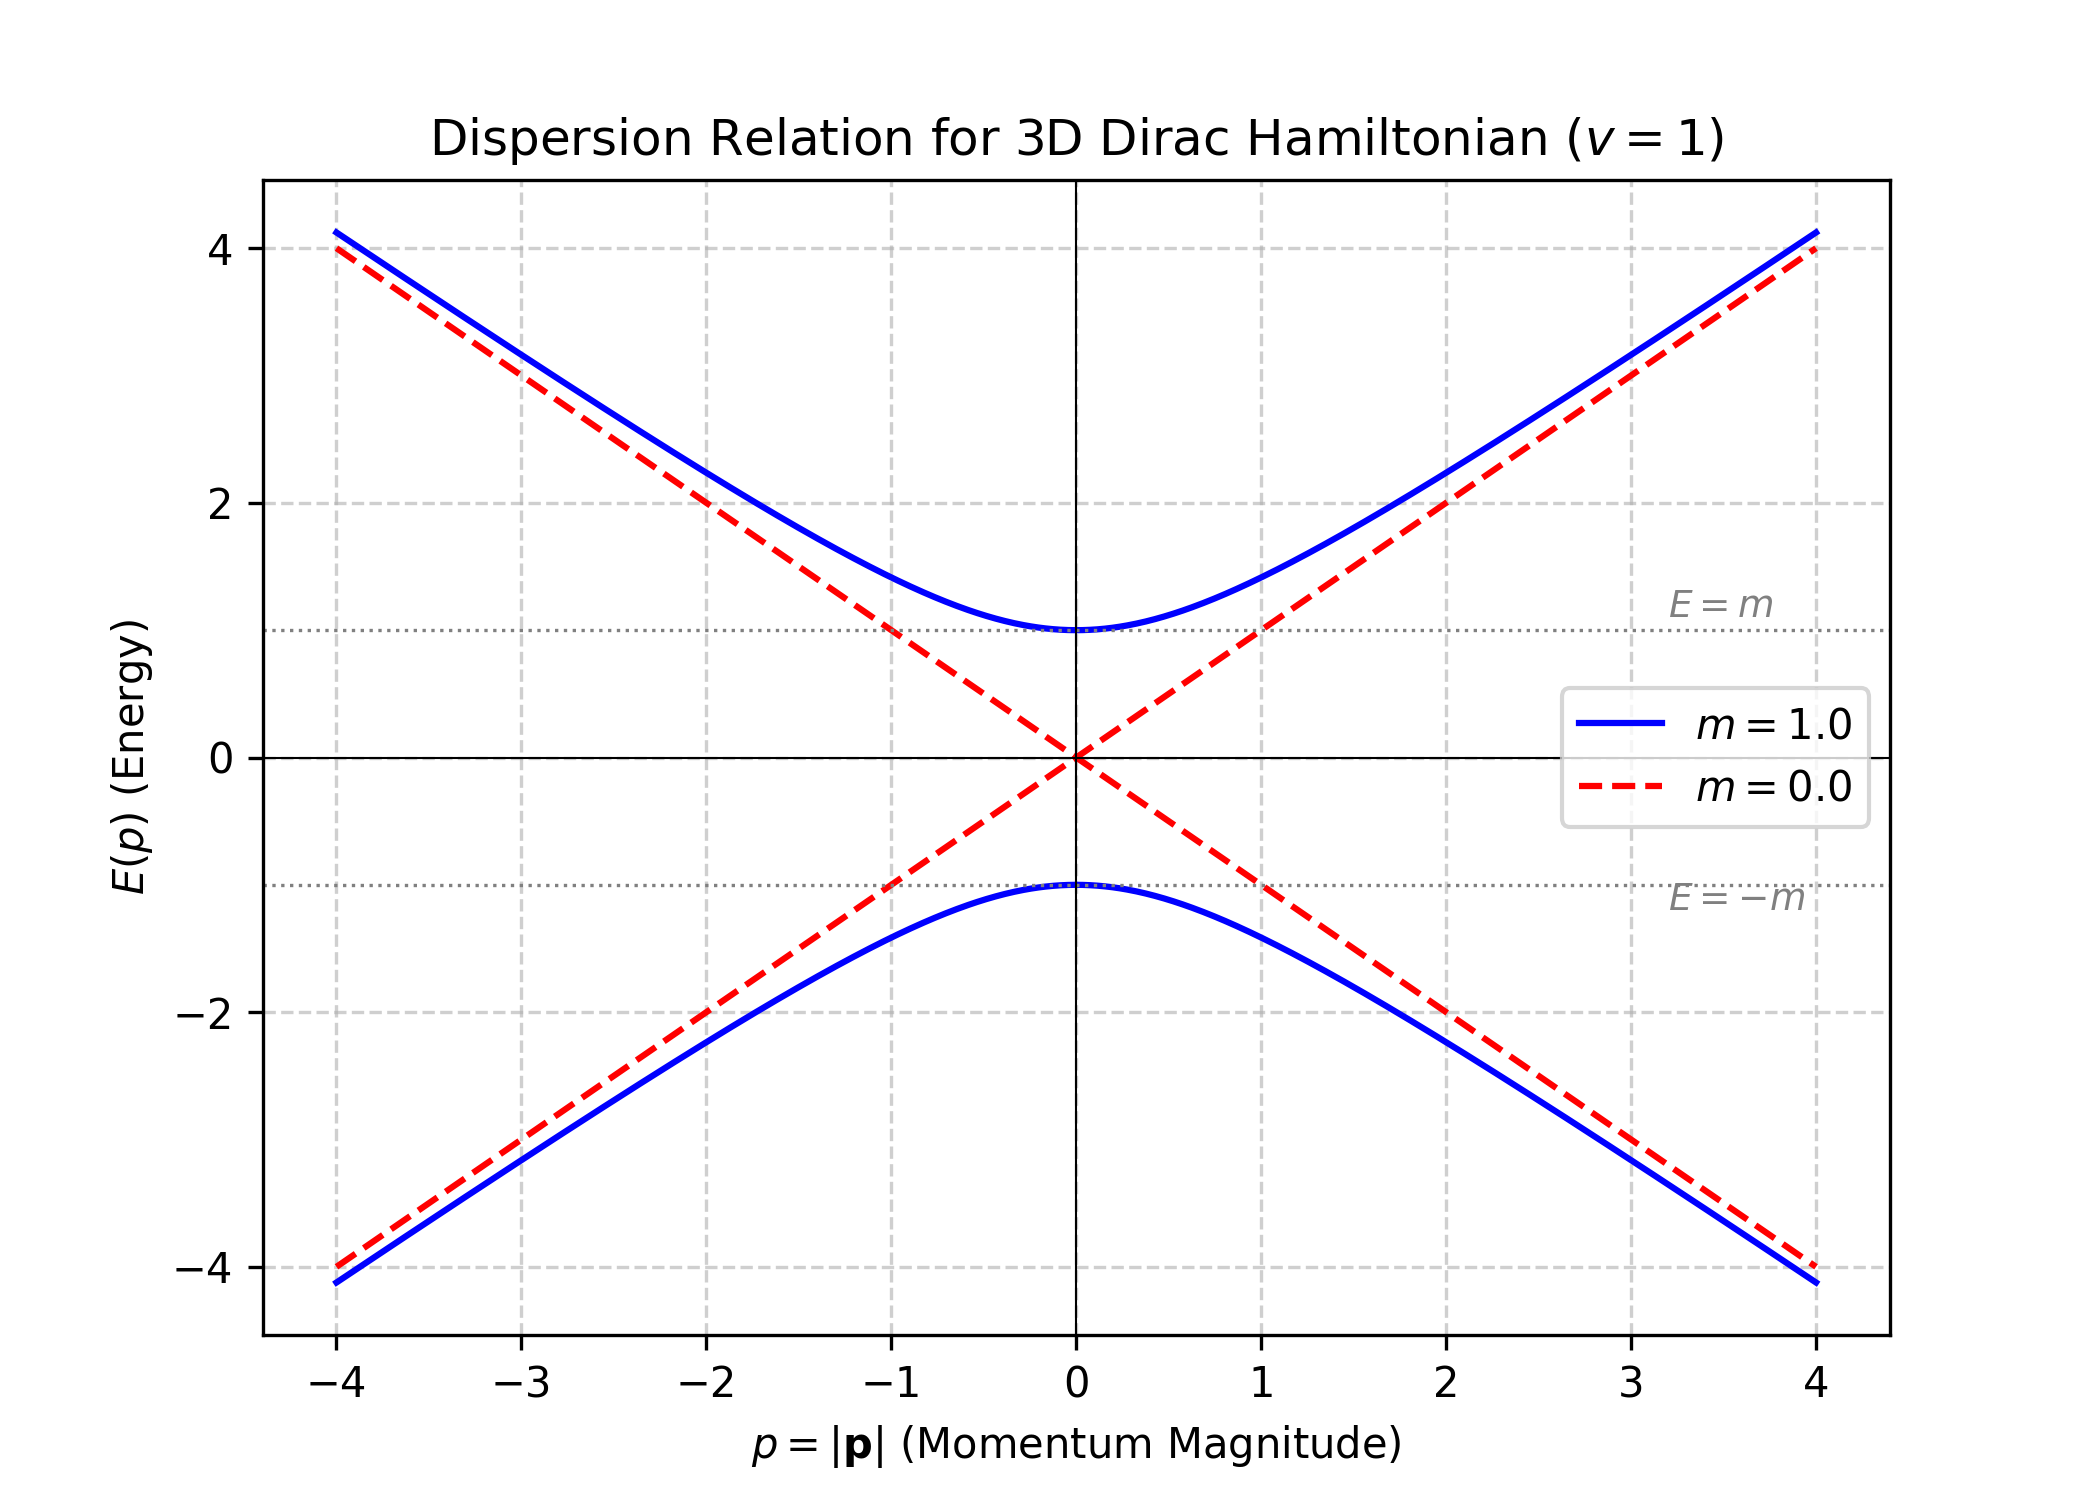
\includegraphics[width=0.7\textwidth]{3d_dirac_dispersion.png} % Using the same plot file as 1D
    \caption{Dispersion relation $E_{\pm}(p) = \pm \sqrt{m^2 + v^2 p^2}$ versus momentum magnitude $p=|\mathbf{p}|$ for the 3D Dirac Hamiltonian \eqref{eq:3D_eigenvalues}, with $v=1$. Each plotted line represents a doubly degenerate energy band (helicity $s=\pm 1$). The solid lines ($m=1$) show the gapped spectrum, while the dashed lines ($m=0$) show the gapless case featuring a 3D Dirac point where the four states converge at $(E=0, \mathbf{p}=0)$.}
    \label{fig:3D_dispersion} % Use a distinct label for the 3D figure context
\end{figure}


\subsection{Berry Connection and Curvature for 2D Dirac Hamiltonian}

We now calculate the Berry connection $\mathcal{A}_i(\mathbf{p})$ and Berry curvature $\Omega(\mathbf{p})$ by returning to the 2D Dirac Hamiltonian $$H_0 = v(p_x \sigma_x + p_y \sigma_y) + m \sigma_z .$$ 

This Hamiltonian can be written as $H_0(\mathbf{p}) = \vec{d}(\mathbf{p}) \cdot \vec{\sigma}$, where the vector is $\vec{d}(\mathbf{p}) = (v p_x, v p_y, m)$. The corresponding positive energy eigenvalue is $E_+(p) = |\vec{d}(\mathbf{p})| = \sqrt{v^2 p^2 + m^2}$, with $p = |\mathbf{p}|$. We focus on the associated normalized positive-energy eigenstate $\psi_+(\mathbf{p})$.

\subsubsection{Berry Connection:}
The Berry connection is defined as 
$$\mathcal{A}_i(\mathbf{p}) = i \langle \psi_+(\mathbf{p}) | \partial_{p_i} | \psi_+(\mathbf{p}) \rangle$$
for $i=x,y$. While this can be computed by direct differentiation of the eigenstate \eqref{eq:2D_eigenstate_plus}, we can also adapt general formulas. For instance, the structure derived in König et al. \cite{PhysRevB.88.035106} (Appendix A.2, Eq. (A.13)-(A.15)) for a general two-level system $H = \vec{d} \cdot \vec{\sigma}$ shows that $\mathcal{A}_i$ takes a specific form dependent on $\vec{d}$ and its derivatives. Applying this structure to our specific $\vec{d}(\mathbf{p}) = (v p_x, v p_y, m)$ yields:
\begin{equation}
\mathcal{A}_x(\mathbf{p}) = \frac{-v^2 p_y}{2 E_+(p) (E_+(p) + m)}, \quad \mathcal{A}_y(\mathbf{p}) = \frac{v^2 p_x}{2 E_+(p) (E_+(p) + m)}.
\label{eq:2D_Berry_Connection_Cited}
\end{equation}

\subsubsection{Berry Curvature:}

The Berry curvature is $\Omega(\mathbf{p}) = \partial_{p_x} \mathcal{A}_y - \partial_{p_y} \mathcal{A}_x$. 

This can be computed directly from \eqref{eq:2D_Berry_Connection_Cited}. Alternatively, we can use the general formula for the Berry curvature of a two-level system $H = \vec{d} \cdot \vec{\sigma}$, given e.g. in Bernevig \& Hughes \cite{bernevig2013topological} (Chapter 8, Eq. (8.6)) as $F_{ij} = \frac{1}{2d^3} \epsilon_{abc} d_a (\partial_i d_b) (\partial_j d_c)$. For our 2D case, we compute $\Omega = F_{xy}$ with $d = E_+(p)$ and $\vec{d} = (v p_x, v p_y, m)$. The non-zero derivatives are $\partial_{p_x} d_1 = v$ and $\partial_{p_y} d_2 = v$. The only non-vanishing term in the sum is $\epsilon_{312} d_3 (\partial_{p_x} d_1) (\partial_{p_y} d_2) = (1)(m)(v)(v) = m v^2$. This yields:
\begin{equation}
  \Omega(\mathbf{p}) = \frac{1}{2 (E_+(p))^3} (m v^2) = \boxed{\frac{m v^2}{2 (m^2 + v^2 p^2)^{3/2}}}.
\label{eq:2D_Berry_Curvature_Cited}
\end{equation}

We can verify this result by comparing it to the calculation in Bernevig \& Hughes \cite{bernevig2013topological} (Chapter 8, Section 8.2.3), who consider the Hamiltonian $H = k_x \sigma_x + k_y \sigma_y + m \sigma_z$ (implicitly setting $v=1$). Their result, Eq. (8.15), is $F_{xy} = \frac{m}{2(k^2 + m^2)^{3/2}}$. If we set $v=1$ in our result \eqref{eq:2D_Berry_Curvature_Cited}, we obtain $\Omega(\mathbf{p})|_{v=1} = \frac{m}{2(m^2 + p^2)^{3/2}}$, which matches the Bernevig \& Hughes result precisely (identifying momentum $p$ with $k$). 



\subsection{The Chern Number}


The Chern number, $C$, is a topological invariant characterizing gapped 2D band structures. It is defined as the integral of the Berry curvature over the Brillouin zone (which is the entire 2D momentum space for a continuum model) with a specific normalization factor. As presented in Bernevig \& Hughes \cite{bernevig2013topological} (Chapter 2.3), the Chern number is:
\begin{equation}
C = \frac{1}{2\pi} \int \Omega(\mathbf{p}) \, d^2p.
\label{eq:ChernDef_Standard}
\end{equation}
This definition is widely used and is consistent with the Hall conductivity formula $\sigma_{xy} = C \frac{e^2}{h}$ (see, e.g., Bernevig \& Hughes \cite{bernevig2013topological} Eq. (3.1) or Eq. (8.16)). 


Using Eq. ~\eqref{eq:2D_Berry_Curvature_Cited}, we can compute the Berry curvature integral in \eqref{eq:ChernDef_Standard}, over the entire 2D momentum space:
\[ \int d^2p \, \Omega(\mathbf{p}) = \int_0^{2\pi} d\phi \int_0^\infty p dp \, \frac{m v^2}{2 (m^2 + v^2 p^2)^{3/2}} = \pi \sgn(m) \]

Subsituting this into the Chern number formula \eqref{eq:ChernDef_Standard} gives:
\begin{equation}
C = \int \frac{d^2 p}{2\pi} \Omega(\mathbf{p}) = \frac{1}{2\pi} \left( \pi \sgn(m) \right) = \boxed{ \frac{1}{2} \sgn(m)}.
\label{eq:2D_Integral_Value_Final}
\end{equation}




\section{Landau Levels for 2D Dirac Hamiltonian}

We investigate the energy spectrum of the 2D Dirac Hamiltonian $H = v(p_x \sigma_x + p_y \sigma_y) + m \sigma_z$ in the presence of a uniform perpendicular magnetic field $\mathbf{B} = B \hat{\mathbf{z}}$. Here, $v$ is the characteristic velocity (analogous to the Fermi velocity $v_F$ in graphene, see Katsnelson \cite{Katsnelson2012Graphene} Chap. 2), and $m$ represents the mass gap energy. We set $\hbar=1$. This model is fundamental for understanding phenomena like the quantum Hall effect in gapped Dirac systems.

\subsection{Canonical Momentum, Ladder Operators, and Hamiltonian Form}
In a magnetic field, the kinetic momentum $\hat{\mathbf{p}}$ is replaced by the canonical momentum $\hat{\mathbf{\Pi}} = \hat{\mathbf{p}} - q\mathbf{A}$, where $q$ is the charge of the particle ($q=-e$ for electrons) and $\mathbf{A}$ is the vector potential such that $\nabla \times \mathbf{A} = \mathbf{B}$. The components of $\hat{\mathbf{\Pi}}$ satisfy the commutation relation $[\hat{\Pi}_x, \hat{\Pi}_y] = i q B$. The resulting energy spectrum is physically independent of the specific gauge choice for $\mathbf{A}$.

Following the standard procedure for Landau levels (see, e.g., König et al. \cite{PhysRevB.88.035106} Appendix A.3 or Katsnelson \cite{Katsnelson2012Graphene} Chap. 2 for the graphene case), we define operators $\hat{\Pi}_{\pm} = \hat{\Pi}_x \pm i \hat{\Pi}_y$. Their commutator is $[-i \hat{\Pi}_-, i \hat{\Pi}_+] = -2qB$.
Ladder operators $b, b^\dagger$ are then constructed:
\begin{itemize}
    \item If $qB < 0$: $b = \frac{i \hat{\Pi}_-}{\sqrt{2|qB|}}$, $b^\dagger = \frac{-i \hat{\Pi}_+}{\sqrt{2|qB|}}$.
    \item If $qB > 0$: $b = \frac{-i \hat{\Pi}_+}{\sqrt{2|qB|}}$, $b^\dagger = \frac{i \hat{\Pi}_-}{\sqrt{2|qB|}}$.
\end{itemize}
These operators satisfy the canonical commutation relation $[b, b^\dagger]=1$, as verified by substituting the definitions of $\hat{\Pi}_{\pm}$ and using $[\hat{\Pi}_x, \hat{\Pi}_y]=iqB$. They act on harmonic oscillator states $|n\rangle$ ($n=0, 1, 2, ...$) such that $b^\dagger b |n\rangle = n |n\rangle$.

The Dirac Hamiltonian $H = v(\hat{\Pi}_x \sigma_x + \hat{\Pi}_y \sigma_y) + m \sigma_z$ can be rewritten in matrix form as 
$$H = \begin{pmatrix} m & v \hat{\Pi}_- \\ v \hat{\Pi}_+ & -m \end{pmatrix}.$$
Substituting $\hat{\Pi}_{\pm}$ and defining the characteristic magnetic energy scale $\Omega_c = v \sqrt{2|qB|}$, we obtain:
\begin{itemize}
    \item If $qB < 0$: \[H = \begin{pmatrix} m & -i \Omega_c b \\ i \Omega_c b^\dagger & -m \end{pmatrix},\]
    \item If $qB > 0$: \[H = \begin{pmatrix} m & -i \Omega_c b^\dagger \\ i \Omega_c b & -m \end{pmatrix}.\]
\end{itemize}
(These matrix forms differ by factors of $\pm i$ from those in \cite{PhysRevB.88.035106} Appendix A.3, which uses a different initial Dirac Hamiltonian structure. However, the eigenvalue spectrum remains the same.)

\subsection{Energy Spectrum and Eigenstates}
To find the energy eigenvalues $E$, we solve $H |\Psi\rangle = E |\Psi\rangle$ by proposing eigenstates that are combinations of harmonic oscillator states $|n\rangle$ coupled with the spinor structure.

\textbf{For Landau Levels $n \ge 1$:}

We seek solutions of the form $|\Psi_n\rangle = (A |n'\rangle, B |n''\rangle)^T$.

If $qB < 0$, using the ansatz $|\Psi_n\rangle = (A |n-1\rangle, B |n\rangle)^T$, the problem reduces to diagonalizing the $2 \times 2$ matrix 
$$\begin{pmatrix} m & -i \Omega_c \sqrt{n} \\ i \Omega_c \sqrt{n} & -m \end{pmatrix}.$$

The characteristic equation $(m-E)(-m-E) - (-i\Omega_c\sqrt{n})(i\Omega_c\sqrt{n}) = 0$ yields $E^2 = m^2 + \Omega_c^2 n$.

A similar procedure for $qB > 0$ with ansatz $|\Psi_n\rangle = (A |n\rangle, B |n-1\rangle)^T$ leads to the same energy relation.

Thus, for $n = 1, 2, 3, ...$, the energy levels are:
\begin{equation}
E_{n, \pm} = \pm \sqrt{m^2 + \Omega_c^2 n} = \boxed{\pm \sqrt{m^2 + 2 v^2 |qB| n}}.
\end{equation}
For each $n = 1, 2, 3, ...$, there are two distinct energy eigenvalues, $E_{n,+}$ and $E_{n,-}$. Each of these energy states (e.g., the state with energy $E_{n,+}$) possesses an orbital degeneracy $N_{deg}$ (discussed in the next subsection). The normalized eigenstates are superpositions of $|n-1\rangle$ and $|n\rangle$ for the two spinor components, with coefficients depending on $E_{n,\pm}, m,$ and $\Omega_c\sqrt{n}$.

\textbf{For the Zeroth Landau Level ($n=0$):}

The $n=0$ harmonic oscillator state satisfies $b|0\rangle=0$.

\begin{itemize}
    \item If $qB < 0$: The Hamiltonian is $H = \begin{pmatrix} m & -i \Omega_c b \\ i \Omega_c b^\dagger & -m \end{pmatrix}$. An eigenstate of the form $\begin{pmatrix} 0 \\ |0\rangle \end{pmatrix}$ yields 
    $$H \begin{pmatrix} 0 \\ |0\rangle \end{pmatrix} = -m \begin{pmatrix} 0 \\ |0\rangle \end{pmatrix}.$$

    \item If $qB > 0$: The Hamiltonian is $H = \begin{pmatrix} m & -i \Omega_c b^\dagger \\ i \Omega_c b & -m \end{pmatrix}$. An eigenstate of the form $\begin{pmatrix} |0\rangle \\ 0 \end{pmatrix}$ yields 
    $$H \begin{pmatrix} |0\rangle \\ 0 \end{pmatrix} = m \begin{pmatrix} |0\rangle \\ 0 \end{pmatrix}.$$
\end{itemize}

Thus, the $n=0$ Landau level has a unique energy:
\begin{equation}
  \boxed{E_0 = m \sgn(qB).}
\end{equation}

The eigenstate for $n=0$ is $(0, |0\rangle)^T$ if $qB<0$ and $(|0\rangle, 0)^T$ if $qB>0$. This means the zeroth Landau level is non-degenerate in the spinor subspace (it involves only one spinor component). This energy spectrum is consistent with the general form presented in König et al. \cite{PhysRevB.88.035106} Eq. (A.22).

\subsection{Degeneracy of Each Landau Level}

The energy eigenvalues $E_{n,\pm}$ and $E_0$ do not depend on the quantum number $k_y$ (momentum in the $y$-direction, conserved in the Landau gauge $\mathbf{A}=(0,Bx,0)$), which dictates the center of the harmonic oscillator wavefunctions $x_0 = k_y/(qB)$.

For a sample of area $A=L_x L_y$, the number of allowed $k_y$ values such that $0 \le x_0 \le L_x$ is:
\[ N_{deg} = \frac{|qB| L_x L_y}{2\pi} = \frac{|qB|A}{2\pi}. \]


Using $\hbar=1$, the flux quantum is $\Phi_0 = 2\pi/|q|$. Thus, the orbital degeneracy of each Landau level $n$ is:
\begin{equation}
N_{deg} = \frac{|B|A}{\Phi_0} = \frac{|\Phi|}{\Phi_0},
\end{equation}

which is the number of flux quanta threading the sample. For physical systems like graphene, this orbital degeneracy would be further multiplied by spin ($g_s=2$) and valley ($g_v=2$) degeneracies (Katsnelson \cite{Katsnelson2012Graphene}, Chap. 2.3). For the simple two-component model considered here, the $n=0$ level (with energy $E_0$) has a total degeneracy of $N_{deg}$. For $n \ge 1$, each distinct energy eigenvalue $E_{n,+}$ and $E_{n,-}$ has an orbital degeneracy of $N_{deg}$.


\subsection{Discussion of Spectrum for Small \texorpdfstring{$n$}{n} vs. Mass Gap \texorpdfstring{$m$}{m}}

The Landau level spectrum $E_{n, \pm} = \pm \sqrt{m^2 + 2 v^2 |qB| n}$ for $n \ge 1$ and $E_0 = m \sgn(qB)$ has distinct features:
\begin{itemize}
    \item \textbf{Massless Case ($m=0$):} $E_{n, \pm} = \pm v \sqrt{2|qB|n}$ for $n \ge 1$, and $E_0 = 0$. The presence of a zero-energy Landau level and the $\sqrt{nB}$ scaling are hallmarks of 2D Dirac fermions, famously observed in graphene (Katsnelson \cite{Katsnelson2012Graphene}, Chap. 2).
    % ... (Massless Case part remains the same) ...
        \item \textbf{Massive Case ($m \neq 0$):}
            \begin{itemize}
                \item When the discrete Landau level energy $2 v^2 |qB| n$ is small compared to the mass gap squared $m^2$ (i.e., for small $n$ or weak $B$ such that $v\sqrt{2|qB|n} \ll |m|$):
                $$E_{n, \pm} \approx \pm \sqrt{m^2(1 + \frac{2 v^2 |qB| n}{m^2})} \approx \pm |m| (1 + \frac{v^2 |qB| n}{m^2}).$$
                The levels are nearly symmetric around $E=0$, starting near $\pm|m|$ for $n=1$. The spacing between adjacent $n$ values on the same energy branch (e.g., $E_{n+1,+} - E_{n,+}$) is approximately $\frac{v^2|qB|}{|m|}$.
                The $n=0$ level is at $m \sgn(qB) = \pm |m| \sgn(m)\sgn(qB)$.
                \item When $v\sqrt{2|qB|n} \gg |m|$ (large $n$ or strong $B$): The $\sqrt{nB}$ behavior dominates, similar to the massless case.
            \end{itemize}
        The $n=0$ level's energy $E_0 = m \sgn(qB)$ is particularly important. Its position relative to $E=0$ depends on the sign of $m$ and $qB$.
    \end{itemize}
    

\subsection{Density of Electrons at Half-Filling (\texorpdfstring{$\mu=0$}{mu=0})}

Furthermore, understanding how the electron density $n$ responds to changes in the magnetic field $B$ and chemical potential $\mu$ is key to describing transport phenomena such as the Hall effect from a thermodynamic perspective \cite{Widom1982}. In the subsequent sections, we will calculate the density at half-filling and its derivative with respect to the magnetic field.

At half-filling (chemical potential $\mu=0$), we sum the contributions of all negative energy states to find the electron density $\bar{n}_0$ (relative to the density at $B=0, m \to \infty$). Each Landau level contributes a density of $g = N_{deg}/A = |qB|/(2\pi)$.

The negative energy states are $E_{n,-} = -\sqrt{m^2 + 2 v^2 |qB| n}$ for $n \ge 1$, and the $E_0$ level if $E_0 = m \sgn(qB) < 0$. The condition $E_0 < 0$ is equivalent to $\sgn(m q B) = -1$.

A direct summation over infinitely many levels diverges. Regularization procedures, such as those discussed in the context of the quantum Hall effect or in Appendix A.3.1 of König et al. \cite{PhysRevB.88.035106}, yield a finite result. The result (Eq. A.28 in \cite{PhysRevB.88.035106}, consistent with our mass convention) is:
\begin{equation}
\bar{n}_0 = -\sgn(qBm) \frac{1}{2} \frac{|B|}{\Phi_0} = -\sgn(qBm) \frac{|qB|}{4\pi}.
\label{eq:half_filling}
\end{equation}

This density arises from the asymmetry introduced by the $n=0$ Landau level. If the $n=0$ level is filled ($E_0 < 0$, which means $\sgn(mqB)=-1$), it effectively contributes an electron density of $g/2 = |qB|/(4\pi)$ relative to a perfectly particle-hole symmetric spectrum (where $g = N_{deg}/A = |qB|/(2\pi)$ is the density of states per LL). If the $n=0$ level is empty ($E_0 > 0$, meaning $\sgn(mqB)=1$), it implies a hole density of $g/2$, or an electron density contribution of $-g/2$.

\subsection[Calculation of d n0/dB]{Calculation of \texorpdfstring{$d\bar{n}_0/dB$}{d n0/dB}}

The rate at which the electron density changes with the magnetic field, $d\bar{n}_0/dB$, is not only a fundamental characteristic of the system but also has direct relevance to transport phenomena like the Hall effect. For instance, thermodynamic arguments by Widom \cite{Widom1982} relate the Hall current to derivatives of the electron density with respect to the magnetic field (cf. Eq. (2) in \cite{Widom1982}). We now calculate this quantity for our 2D Dirac system at half-filling.

The density of electrons at half-filling, given by Eq. ~\ref{eq:half_filling}, is
$$ \bar{n}_0 = -\sgn(qBm) \frac{|qB|}{4\pi}. $$
We can rewrite this expression by noting that $\sgn(x)|x| = x$.
Thus, $\sgn(qB)|qB| = qB$. The term $\sgn(qBm)$ can be written as $\sgn(qB)\sgn(m)$.
So,
$$ \bar{n}_0 = -\sgn(m) \sgn(qB) \frac{|qB|}{4\pi} = -\sgn(m) \frac{qB}{4\pi}. $$
This expression for $\bar{n}_0$ is linear in the magnetic field $B$.

Differentiating this form of $\bar{n}_0$ with respect to $B$ (for $B \neq 0$) yields:
\begin{equation}
\boxed{
\frac{d\bar{n}_0}{dB} = -\frac{q \sgn(m)}{4\pi}.}
\end{equation}

This quantity represents the rate at which the electron density (relative to the $B=0, m \to \infty$ reference) changes with the magnetic field to keep the chemical potential at $\mu=0$. It is a constant that depends on the charge $q$ and the sign of the mass gap $m$. Unlike a function with a cusp at $B=0$, this derivative is well-defined and constant for $B \neq 0$. The behavior exactly at $B=0$ is special as Landau levels themselves are not formed, but the derived density $\bar{n}_0(B)$ is a smooth function through $B=0$.



% --- Bibliography ---
\begin{thebibliography}{9}

\bibitem{bernevig2013topological} % Add if citing Bernevig again
B. A. Bernevig and T. L. Hughes,
\textit{Topological Insulators and Topological Superconductors}
(Princeton University Press, Princeton, NJ, 2013).

\bibitem{Katsnelson2012Graphene}
M. I. Katsnelson,
\textit{Graphene: Carbon in Two Dimensions}
(Cambridge University Press, Cambridge, 2012).

\bibitem{PhysRevB.88.035106}
E. J. K\"onig, P. M. Ostrovsky, I. V. Protopopov, I. V. Gornyi, I. S. Burmistrov, and A. D. Mirlin,
\textit{Interaction and disorder effects in three-dimensional topological insulator thin films},
Phys. Rev. B \textbf{88}, 035106 (2013).
DOI: \href{https://doi.org/10.1103/PhysRevB.88.035106}{10.1103/PhysRevB.88.035106}.

\bibitem{Widom1982}
A. Widom,
\textit{Thermodynamic derivation of the Hall effect current},
Phys. Lett. A \textbf{90}, 474 (1982).
DOI: \href{https://doi.org/10.1016/0375-9601(82)90520-X}{10.1016/0375-9601(82)90520-X}.

\end{thebibliography}






\end{document}